%%%%%%%%%%%%%%%%%%%%%%%%%%%%%%%%%%%%%%%%%%%%%%%%%%%%%%%%%%%%%%%%%%%%%%%%%%%%%%%%
\chapter{An example chapter}
%%%%%%%%%%%%%%%%%%%%%%%%%%%%%%%%%%%%%%%%%%%%%%%%%%%%%%%%%%%%%%%%%%%%%%%%%%%%%%%%

\chapterprecis{You can include a precis: a short summary of the chapter's
               contents (think of \emph{Winnie the Pooh}). There is an option
               in the front-matter to keep the precis out of the table of
               contents; it's included by default!}

Here you'll include everything you want to share with the world, as well as how
it relates to past knowledge \cite{armitage1901}.


You can include figures:

\begin{figure}[ht]
    \centering
    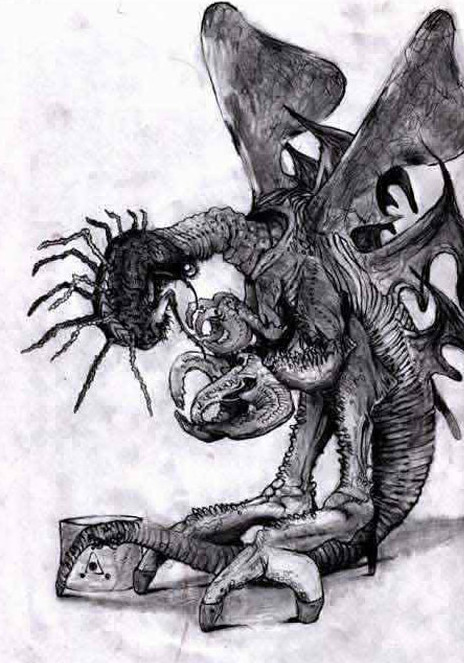
\includegraphics[height=2in]{Migo.jpg}
    \caption[Migo]
            {Migo, drawn by
            \href{https://www.artstation.com/khanneasuntzu}
                 {Khannea SunTzu} and available at 
             \href{https://commons.wikimedia.org/wiki/File:Migo.jpg}
                  {Wikimedia Commons}
            under a CC-BY-SA license.}
    \label{fig:migo}
\end{figure}

and tables:

\begin{table}[ht]
\begin{tabular}{@{}lllll@{}}
    \toprule
    Header 1 & and a second & 3rd & 4th & why so many? \\
    \midrule
    Asteroid & Example data & Etc. & n/a & n/a \\
    Cow & Sphere (?) & n/a & Loud (moo) & n/a \\
    \bottomrule
\end{tabular}
\caption[Cow and Co.]{Various nonsensical data were gathered.}
\label{tab:cow}
\end{table}

and even equations, like this rather famous one. (This uses a macro
from the included package!)
\begin{equation}
    - i \hbar \partial_t \ket{\psi} = H \ket{\psi}.
\end{equation}

Here is a bunch of text so you can see what multiple pages of chapter looks like.

\lipsum[1-19]